\section{Escopo}

Esta seção define a estratégia de aproximação em \gls{rvdb}, tomando como referência a sequência de fases apresentada por \cite{fehse2003}.
O escopo limita-se à caracterização das fases operacionais e aos critérios de transição entre etapas.
A estrutura segue a decomposição por fases ilustrada na Figura~\ref{fig:etapas_rvdb}.
Após a apresentação das etapas, são incluídos comentários específicos sobre os vínculos e condicionantes relevantes em cada fase.
Em particular, na etapa de injeção orbital, discute-se o requisito de compatibilidade geométrica entre as órbitas do perseguidor e do alvo, com ênfase no problema de coplanaridade e em suas implicações para o planejamento da janela de lançamento e para correções subsequentes de trajetória.

\begin{figure}[ht]
\centering

\includegraphics[width=1\linewidth]{3 Formulacao matematica/Imagens/Lançamento quadro explicativo.png}
\caption{Fases de uma missão de \gls{rvdb}, adaptado de \cite{fehse2003}.}
\label{fig:etapas_rvdb}
\end{figure}

%%%%%%%%%%%%%%%%%%%%%%%%%%%%%%%%%%%%

\subsection{Lançamento: vínculos associados às missões de \gls{rvdb}}
\label{sec:lancamento_vinculos}

O início de uma missão de \gls{rvdb} ocorre na etapa de lançamento, conforme ilustrado na Figura~\ref{fig:etapas_rvdb}.
Nessa fase, a espaçonave perseguidora deve ser injetada em uma órbita compatível com a do alvo, considerando a janela de lançamento planejada, de modo a evitar inserções que demandem correções adicionais de trajetória.

A definição da janela de lançamento é vinculada à órbita conhecida do alvo.
Os parâmetros de injeção são escolhidos em função dessa órbita, com o objetivo de garantir a inserção do veículo em uma trajetória coplanar à do alvo, reduzindo a necessidade de manobras posteriores para correção do plano orbital.

%%%%%%%%%%%%%%%%%%%%%%%%%%%%%%%%%%%%%%%%%%%%%%%%%%%%%%%%%%%%%%%%%%%%%%%%%%%%%%%%%%%%%%%%%%%%%%%%%%%%%%%%%%%%

\section{Fases da missão de RVD/B}

A missão considerada neste trabalho segue o encadeamento das operações de \gls{rvdb} entre uma espaçonave perseguidora e uma espaçonave alvo em órbita circular \cite{fehse2003}. Nessas etapas acontecem:

\begin{enumerate}[label=(\roman*)]
  \item lançamento e injeção do perseguidor em sua órbita;
  \item redução da diferença do ângulo de fase entre as espaçonaves;
  \item aproximação de longa distância, através da transferência de órbita do perseguidor;
  \item movimento relativo das espaçonaves, onde ocorrem as aproximações curta distância e final;
  \item ainda nesta fase de aproximação de curta distância e aproximação final, a dinâmica da atitude e órbita da espaçonave robótica é controlada mantendo a sincronização de atitude do perseguidor e da espaçonave alvo.
\end{enumerate}

%%%%%%%%%%%%%%%%%%%%%%%%%%%%%%%%%%%%%%%%%%%%%%%%%%%%%%%%%%%%%%%%%%%%%%%%%%%%%%%%%%%%%%%%%%%%%%%%%%%%%%%%%%%%

\section{Descrição das fases da missão de RVD/B e premissas adotadas}

Adotou-se nessa pesquisa a premissa de que o lançador realiza a injeção do perseguidor em uma órbita circular e coplanar à órbita do alvo.
Essa premissa é discutida à luz da janela de lançamento que pode garantir a injeção com precisão em termos de coplanaridade.

\subsection{Órbita inicial}
\label{sec:fases_orbita_inicial}

Assume-se nesta pesquisa que a órbita de injeção implementada pelo lançador coloque a espaçonave perseguidora em um órbita circular e $500$~km de altitude, coplanar à da espaçonave alvo. 
Em análises de \gls{rvdb}, é comum assumir que o perseguidor é injetado em uma órbita circular e estável.
Isto elimina complicações de excentricidade e facilita o uso de modelos clássicos de mecânica orbital, como \gls{hcw}.

A altitude selecionada está dentro da faixa típica de \gls{leo}, onde muitas missões de \gls{rvdb} ocorrem, como exemplo, a \gls{iss}, está entre $370$--$460$~km \cite{ISSaltitude}.
Optou-se por $500$~km, pois reduz o arrasto atmosférico em comparação a altitudes menores, mas ainda mantém o ambiente acessível para lançadores.
Por sua vez, o veículo perseguidor pode ser injetado em uma órbita circular próxima à do alvo, e a partir daí realizar manobras orbitais de faseamento e aproximação.
Esse cenário é didático e consistente com a literatura de \gls{rvdb}, que frequentemente parte de órbitas circulares coplanares como condição inicial.

Após a injeção do perseguidor em sua órbita inicial, a aproximação longa é iniciada.
Nesta fase, o movimento do perseguidor é descrito no referencial inercial.

\begin{figure}[H]
\centering

\includegraphics[width=1\linewidth]{2 Estrategia de RVDB/Imagens/1 Posicao espaconaves injecao orbital.png}
\caption{Posição relativa das espaçonaves no momento da injeção do perseguidor em sua órbita inicial.}
\label{fig:injecao_orbita_inicial}
\end{figure}

%%%%%%%%%%%%%%%%%%%%%%%%%%%%%%%%%%%%%%%%%%%%%%%%%%%%%%%%%%%%%%%%%%%%%%%%%%%%%%%%%%%%%%%%%%%%%%%%%%%%%%%%%%%%

\subsection{Transferência de órbita}
\label{sec:fases_transf_orbita}

Ao reduzir a diferença de ângulo entre as espaçonaves, é realizada a transferência de órbita através de duas manobras impulsivas (do tipo Hohmann) que o conduzem para a nova órbita, possuindo raio orbital também inferior ao do alvo.
Além disso, o perseguidor estará atrasado em relação ao alvo, tanto em sua óbita inicial como na nova órbita após terminada a transferência orbital.

\begin{figure}[H]
\centering

\includegraphics[width=1\linewidth]{2 Estrategia de RVDB/Imagens/2 Posicao espaconaves antes da transf de orbita.png}
\caption{Posição relativa das espaçonaves no momento de início da transferência de órbita do perseguidor.}
\label{fig:transf_orbita}
\end{figure}

A Figura~\ref{fig:fases_RVDB} ilustra a posição da espaçonave alvo e a movimentação relativa realizada pelo perseguidor.

\begin{figure}[H]
\centering

\includegraphics[width=1\linewidth]{2 Estrategia de RVDB/Imagens/3 Sequencia das fases.png}
\caption{Diagrama das fases da missão de \gls{rvdb}.}
\label{fig:fases_RVDB}
\end{figure}

Os números presentes nesta Figura contribuem com o entendimento da sequência realizada:
(1) o perseguidor após a injeção em sua órbita inicial realiza a deriva orbital para reduzir o ângulo de fase;
(2) transferência de órbita;
(3) acomodação do perseguidor em sua nova órbita e realizará uma nova deriva orbital enquanto faz checagens de posição e velocidade;
(4) início do movimento relativo no referencial local, centrado no alvo.

%%%%%%%%%%%%%%%%%%%%%%%%%%%%%%%%%%%%%%%%%%%%%%%%%%%%%%%%%%%%%%%%%%%%%%%%%%%%%%%%%%%%%%%%%%%%%%%%%%%%%%%%%%%%

\subsection{Aproximação de curta distância}
\label{sec:fases_app_curta}

Para realizar nova translação do perseguidor, utilizaram-se as equações linearizadas de \gls{hcw}, juntamente com uma lei de \gls{pd} para garantir acurácia na manobra e que toda a movimentação seja suave, ambas no referencial \gls{lvlh}.
No mesmo instante, devido a maior proximidade com o alvo, os sensores do perseguidor realizam a leitura da atitude do alvo e comparam com a sua própria atitude para que outra lei de controle \gls{pd} implementada possa realizar a correção.
A nova posição relativa desejada do perseguidor é inferior a um metro abaixo da porta de acoplamento do alvo.

%%%%%%%%%%%%%%%%%%%%%%%%%%%%%%%%%%%%%%%%%%%%%%%%%%%%%%%%%%%%%%%%%%%%%%%%%%%%%%%%%%%%%%%%%%%%%%%%%%%%%%%%%%%%

\subsection{Aproximação final}
\label{sec:fases_app_final}

No instante em que o perseguidor atingir essa nova posição relativa em relação ao alvo, ele estará alinhado em termos de atitude, permitindo que o \gls{eef} possa ser alinhado com a porta de acoplamento.

\begin{figure}[H]
\centering
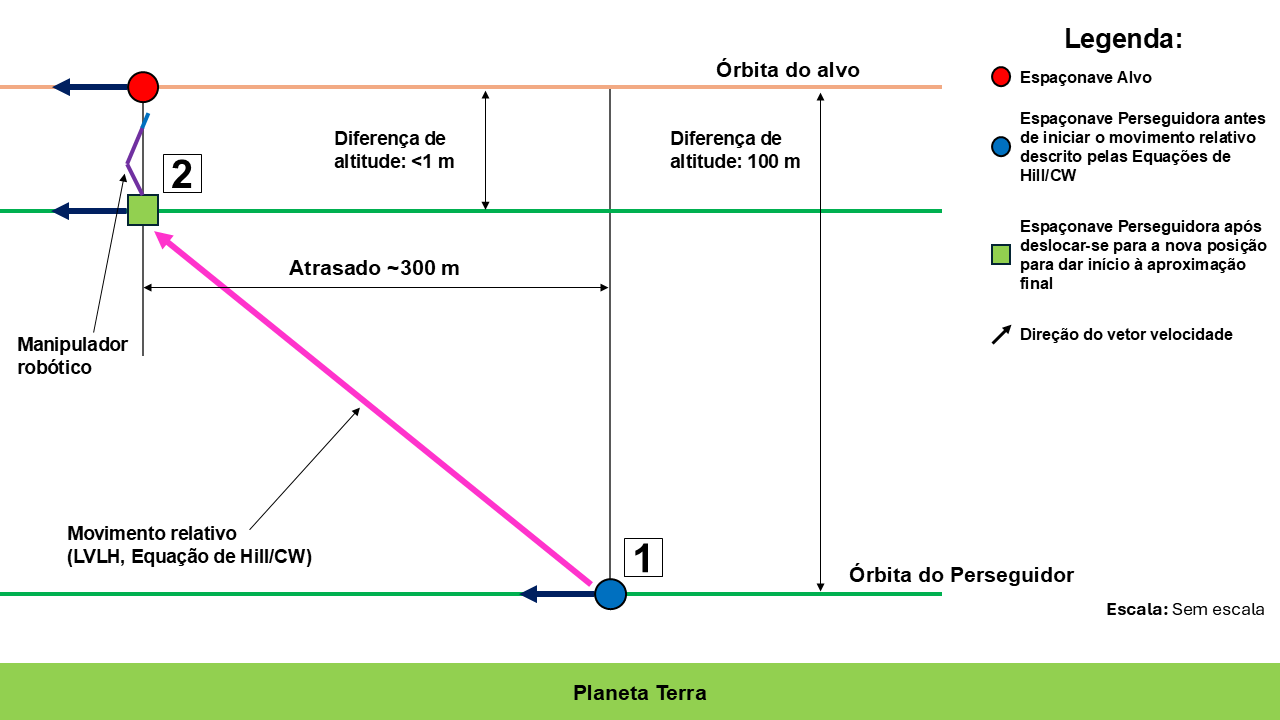
\includegraphics[width=1\linewidth]{2 Estrategia de RVDB/Imagens/4 App final.png}
\caption{Diagrama da aproximação final da missão de RVD/B.}
\label{fig:app_final}
\end{figure}

A Figura~\ref{fig:app_final} ilustra o momento em que o perseguidor vai (1) iniciar a aproximação curta através da \gls{hcw}, e (2) onde ele irá movimentar o \gls{mr} após a sua estabilização total, tanto de atitude como de posição e velocidade relativa, para engatar a \gls{eef} na porta de acoplamento do alvo.

%%%%%%%%%%%%%%%%%%%%%%%%%%%%%%%%%%%%%%%%%%%%%%%%%%%%%%%%%%%%%%%%%%%%%%%%%%%%%%%%%%%%%%%%%%%%%%%%%%%%%%%%%%%%

\subsubsection{Movimentação do manipulador robótico}

Nesta fase de aproximação final, após o sistema de controle estabilizar a pose do perseguidor e o manipulador entrar no modo operacional, o \gls{mr} irá iniciar a sua movimentação para alinhar o \gls{eef} com a porta de acoplamento no eixo radial do alvo.
Durante a operação do \gls{mr}, torques e forças de reação são transmitidos a espaçonave perturbando sua atitude e posição.

O controle ativo da atitude relativa atua para corrigir os efeitos dinâmicos introduzidos pelo movimento do manipulador. A rotação das juntas e o consequente deslocamento do centro de massa geram torques que podem provocar reposicionamentos instantâneos na órbita, resultando em desalinhamentos angulares da atitude e pequenos desvios do centro de massa em relação à trajetória nominal.
Esses efeitos devem ser prontamente anulados pelo sistema de controle de órbita e de atitude, de modo a preservar a estabilidade global da manobra.

%%%%%%%%%%%%%%%%%%%%%%%%%%%%%%%%%%%%%%%%%%%%%%%%%%%%%%%%%%%%%%%%%%%%%%%%%%%%%%%%%%%%%%%%%%%%%%%%%%%%%%%%%%%%

\section{Modos de operação e referenciais}

Para cada fase da missão de \gls{rvdb} apresentada foram utilizados diferentes modos de operação do \gls{mr} e referenciais (sistemas de coordenadas).
Foram estabelecidos dois modos de operação do \gls{mr}: não-operacional e operacional.
A Tabela~\ref{tab:modos_operacao} apresenta os modos e quando são utilizados durante a missão de \gls{rvdb}.

\begin{table}[htbp]
\centering
\caption{Modos de operação e respectivas descrições.}
\label{tab:modos_operacao}
\begin{tabular}{p{0.25\linewidth} p{0.67\linewidth}}
\hline
\textbf{Modo de operação} & \textbf{Descrição} \\
\hline
Não-operacional &
% Neste modo, inicia-se o controle de atitude relativa. Concluída a manobra de aproximação de curta duração, o controle de atitude deve manter a espaçonave perseguidora alinhada e permitir o início da aproximação de proximidade. Nesse estágio, o controle de atitude relativa precisa garantir um ajuste fino, eliminando os efeitos de reação do manipulador sobre a espaçonave.\\
Esse modo corresponde à configuração da espaçonave tipo \gls{mr} com elos dobrados e travados.
Permance nessa configuração durante o lançamento, injeção em órbita e fica nessa configuração até a aproximação final.
Essa estratégia é importante porque durante todo esse tempo o modelo da dinâmica orbital e de atitude  é o de corpo rígido, valendo as equações de Euler para a dinâmica de atitude.\\
\hline
Operacional &
% No instante que a aproximação final é iniciada, troca-se para a dinâmica acoplada, que utiliza as equações de Lagrange para esta finalidade. \\
Imediatamente antes do início da aproximação de proximidade (aproximação final), o \gls{mr} é destravado, entrado no Modo Operacional.
Esse modo torna a dinâmica mais complexado o modelo da dinâmica tem que ser descrito pelas equações modificads de Euler que são obtidas então, via abordagem Lagrangiana.\\
\hline
\end{tabular}
\end{table}

%%%%%%%%%%%%%%%%%%%%%%%%%%%%%%%%%%%%%%%%%%%%%%%%%%%%%%%%%%%%%%%%%%%%%%%%%%%%%%%%%%%%%%%%%%%%%%%%%%%%%%%%%%%%

\subsection{Referenciais}

Por sua vez, a Tabela~\ref{tab:fases_missao_referenciais} exibe cada fase da missão de \gls{rvdb} e qual sistema de coordenada foi utilizado.

\begin{table}[H]
\centering
\caption{Fases da missão, tipo de movimento e referencial associado.}
\label{tab:fases_missao_referenciais}
\begin{tabular}{lll}
\hline
\textbf{Fase da missão} & \textbf{Tipo} & \textbf{Referencial} \\
\hline
Injeção orbital         & Movimento absoluto & ECI \\
Órbita de fase          & Movimento absoluto & ECI \\
Transferência de órbita & Movimento absoluto & ECI \\
Aproximação final & Movimento relativo & LVLH \\
Aproximação curta & Movimento relativo & LVLH \\
\hline
\end{tabular}
\end{table}

% A seguir serão detalhadas as leis de controle utilizada em todas as fases da missão de \gls{rvdb} deste trabalho.

%%%%%%%%%%%%%%%%%%%%%%%%%%%%%%%%%%%%%%%%%%%%%%%%%%%%%%%%%%%%%%%%%%%%%%%%%%%%%%%%%%%%%%%%%%%%%%%%%%%%%%%%%%%%

\section{Estratégia de controle de atitude}
\label{sec:controle_atitude}

% A estratégia de controle adotada combina uma lei de controle aplicado à dinâmica relativa em \gls{lvlh} com outra lei de controle atribuída à correção da atitude da espaçonave.
% Esta abordagem é usada nos dois modos de operação definidos (não operacional e operacional) do \gls{mr}.
O sistema de controle opera em dois modos distintos:
(1) quando o manipulador robótico estiver travado (descrito pela dinâmica de corpo rígido) e
(2) quando o \gls{mr} estiver em operação (descrito pela dinâmica acoplada da atitude e variáveis do movimento do \gls{mr}).
Na fase de aproximação final, uma lei de controle atua nas juntas do manipulador para executar a manobra de captura.
A estratégia inclui também os pontos de referência (\emph{waypoints}), que são pontos de espera para possíveis ajustes de posição e velocidades e cheques de segurança do sistema robótico.
% A transição entre cada fase da missão apresentadas na Seção~\ref{sec:fases_orbita_inicial} ocorre quando são satisfeitos os seguintes critérios:

% \begin{enumerate}[label=(\roman*)]
%   \item distância relativa das espaçonaves inferior a um limite estabelecido para a etapa da missão de \gls{rvdb};
%   \item correto alinhamento da atitude do perseguidor em relação à atitude do alvo, dentro de um limite estabelecido.
% \end{enumerate}

\subsection{Controle PD na dinâmica relativa}
\label{sec:controle_PD_HCW}

A aproximação relativa no referencial \gls{lvlh}, definido no centro de massa da espaçonave alvo, é descrita pelo modelo linearizado \gls{hcw}.
Neste referencial é descrito o movimento relativo entre a espaçonave perseguidora e a espaçonave alvo.
A abordagem de controle do movimento orbital relativo é realizado pela lei de controle \gls{pd}.
O objetivo é conduzir o movimento relativo a um órbita cuja deriva possa ser utilizada para reduzir um ângulo de fase que atenda a condição de aproximação final com o \gls{mr} em modo não operacional. 

%%%%%%%%%%%%%%%%%%%%%%%%%%%%%%%%%%%%%%%%%%%%%%%%%%%%%%%%%%%%%%%%%%%%%%%%%%%%%%%%%%%%%%%%%%%%%%%%%%%%%%%%%%%%

\subsection{Controle de atitude durante o modo não operacional do \gls{mr}}
\label{sec:controle_atitude_Euler}

No modo não operacional, a \gls{etmr} é tratada como corpo rígido.
A estratégia consiste em aplicar a técnica \gls{pd} para controle da atitude descrita em quaternion de erro entre a orientação da espaçonave perseguidora e uma orientação de referência associada ao alvo medida no sistema corpo.
O controle é responsável por manter o perseguidor alinhado com o alvo durante a aproximação curta, enquanto o controle translacional define a trajetória relativa.

%%%%%%%%%%%%%%%%%%%%%%%%%%%%%%%%%%%%%%%%%%%%%%%%%%%%%%%%%%%%%%%%%%%%%%%%%%%%%%%%%%%%%%%%%%%%%%%%%%%%%%%%%%%%

\subsection{Controle de atitude durante o modo operacional do \gls{mr}}
\label{sec:controle_atitude_Lagrange}
% 
No modo operacional, o \gls{mr} passa a se movimentar para engatar o \gls{eef} na porta de acoplamento.
A dinâmica do sistema deixa de ser equivalente à de um corpo rígido e passa a ser descrita pela formulação de Lagrange com coordenadas generalizadas que incluem a atitude da base e as juntas do \gls{mr}.
Os movimentos articulares geram torques internos que aparecem como reações na base, alterando a sua atitude.

A estratégia de controle utiliza o mesmo controlador que estabiliza a atitude quando o \gls{mr} está travado, e então passa a atuar também como compensador das reações provenientes dos movimentos das juntas.
Assim, o controle de atitude deve ao mesmo tempo seguir a referência de atitude em relação ao alvo e anular os efeitos dos torques e forças de reação na plataforma robótica.

%%%%%%%%%%%%%%%%%%%%%%%%%%%%%%%%%%%%%%%%%%%%%%%%%%%%%%%%%%%%%%%%%%%%%%%%%%%%%%%%%%%%%%%%%%%%%%%%%%%%%%%%%%%%

\subsection{Síntese das estratégias de controle}


Por fim, a Tabela~\ref{tab:locais_atuacao_controladores} apresenta a forma de implementação da lei de controle \gls{pd} neste trabalho, onde e como cada uma atua, de forma a cumprir a missão de \gls{rvdb}.

\begin{table}[H]
\centering
\caption{Estratégia da lei de controle implementada.}
\label{tab:locais_atuacao_controladores}
\begin{tabular}{p{0.32\linewidth} p{0.62\linewidth}}
\hline
\textbf{Local de atuação} & \textbf{Como atua} \\
\hline
Controle de órbita &
Reduz o erro e mantém a acurácia da posição relativa entre as espaçonaves e translada o perseguidor para próximo do alvo durante a aproximação curta. \\
\hline
Atitude relativa &
Durante as aproximações curta distância e final, mantém a atitude do perseguidor sincronizada com a do alvo. \\
\hline
Juntas do \gls{mr} &
Realiza a movimentação do \gls{mr} para que o efetuador final seja conduzido até a porta de acoplamento, de maneira suave e controlada. \\
\hline
\end{tabular}
\end{table}